\chapter[Conocimientos previos]{Conocimientos previos sobre las tecnologías usadas.}\label{cap:conocimientos}
\markboth{CAPÍTULO \ref{cap:conocimientos}. CONOCIMIENTOS PREVIOS.}{}

En este segundo capítulo vamos a explicar cuáles son las ideas previas de las que partimos y los conocimientos que poseíamos sobre las tecnologías que hemos usado en el proyecto. Haciendo una breve explicación sobre su funcionamiento, su uso, su historia y sus recientes versiones.

El principal elemento usado en el proyecto es el lenguaje de programación Java, que lo hemos usado para programar tanto la aplicación web como la aplicación en el móvil. Pero aparte de los diferentes SDK de Android y de Google App Engine, hemos recurrido y empleado muchas otras tecnologías y lenguajes como pueden ser SQL, XML, UML, GIT. Además hemos aplicado los conocimientos básicos sobre criptografía de clave pública necesarios para realizar todo el proceso de firma digital.   

\section{El lenguaje de programación Java}

Java es un lenguaje de programación orientado a objetos que fue diseñado por James Gosling\footnote{ Para más información sobre James Gosling: \url{http://en.wikipedia.org/wiki/James\_Gosling}} para Sun Microsystems y que recientemente ha sido comprado por Oracle Corporation. Fue lanzado en 1995 y ha sido el centro de toda la plataforma Java de Sun Microsystems. Es un lenguaje con una sintaxis muy parecida a C o C++, pero con la gran ventaja de que el manejo de punteros y objetos es automático, al igual que la recogida de basura.

Java es un lenguaje en el que hay que compilar los códigos fuentes para crear unos archivos intermedios llamados bytecodes, los archivos *.class, que luego serán interpretados por la máquina virtual de Java (JVM). Esta dependerá de la arquitectura en la que se quiera ejecutar la aplicación Java. Gracias a esto se puede decir que Java es un lenguaje multiplataforma, lo que significa que un mismo código Java se puede ejecutar en Linux, en Windows, en Mac o cualquier otro sistema para el cual exista una máquina virtual, lo que en inglés se llama ``write once, run anywhere" (WORA). Además de esta importante ventaja Java es un lenguaje de propósito general, concurrente, basado en clases y orientado a objetos. Java es el segundo lenguaje de programación más popular de 2012, gracias a las aplicaciones web cliente-servidor que tienen tanto auge en estos momentos, como podemos ver en la figura \ref{fig:indicetiobe}.

\begin{figure}[h]
  \centering
    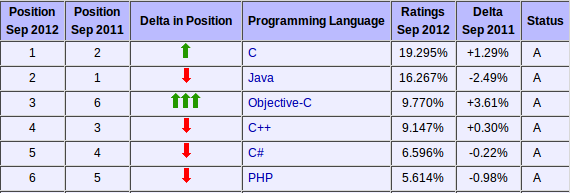
\includegraphics[scale=0.9]{./ConocimientosPrevios/imagenes/indiceTiobe.png}
  \caption{Índice Tiobe en septiembre del 2012. \url{http://www.tiobe.com/}}
  \label{fig:indicetiobe}
\end{figure} 

La implementación original y las referencias del compilador de Java, máquinas virtuales y las librerías de clases fueron desarrolladas por Sun en 1995, pero en el 2007 gracias a la contribución de la comunidad, Sun Microsystems cambió la licencia de todas las tecnologías Java a GNU General Public License, por lo que se abría la posibilidad de que se crearan versiones alternativas de compiladores bajo licencia GNU como por ejemplo GNU Compiler para Java o GNU Classpath.

En el proyecto la versión usada fue la versión \textbf{Java SE}.

\subsection{Historia}

Originalmente Java nació como un proyecto de James Gosling, Mike Sheridan y Patrick Naughton en 1991 y estaba diseñado para una televisión interactiva, pero era muy avanzado para lo que la industria televisiva de la época podía necesitar. En su origen fue llamado Oak, pero por problemas con el nombre, ya que era una marca registrada de otra empresa, lo cambiaron a Green y posteriormente ya lo renombraron al definitivo Java. Hay muchas teorías sobre por qué se llama Java, pero una de ellas es que había una cafetería llamada Java Coffe donde James, Mike and Patrick pasaron muchas horas consumiendo café.

La idea de Gosling era crear una máquina virtual donde funcionara un lenguaje de programación con la sintaxis y la estructura de C/C++ para que la curva de aprendizaje fuera muy suave para los programadores que en la época sabían C/C++.

Sun Microsystems lanzó Java 1.0 en 1995, con la principal característica de que una vez escrito un código fuente no había que modificarlo para que funcionara en las diferentes máquinas, lo que anteriormente hemos llamado con el acrónimo en inglés WORA (Write Once, Run Anywhere). Rápidamente todos los navegadores de la época empezaron a soportar applets Java en las páginas web, por lo que Java se volvió muy popular en la época. La nueva versión Java 2 fue lanzada en 1998-1999 y con ella llegaron las distinciones en diferentes plataformas, como por ejemplo Java2EE para aplicaciones corporativas o una versión ligera llamada Java2ME que estaba diseñada para funcionar en los diferentes teléfonos de la época, y el resto se agrupan en la versión Java2SE, que es la versión estándar.

En 1997, Sun Microsystems intentó formalizar Java mediante una norma ISO/IEC pero se retiró del proceso y dio todo el control a la comunidad. Sun ofrecia implementaciones gratuitas y generaba dinero vendiendo algunas licencias de productos como Java Enterprise System. Una cosa importante es que Sun distingue entre el SDK (Kit de desarrollo) y el JRE (Entorno de ejecución) en el que van incluidos los compiladores, debuggers, etc.

El 13 de noviembre del 2006, Sun lanzó Java gratis y como software libre, bajo la licencia GNU General Public License (GPL). El proceso finalizó el 8 de mayo del 2007.

En 2009-2010 Oracle Corporation compró Sun Microsystems por lo que Java actualmente pertenece a Oracle Corporation.

\subsection{Versiones}

\begin{itemize}

	\item \textbf{JDK 1.0} (23 de enero de 1996): Primer lanzamiento
	
	\item \textbf{JDK 1.1} (19 de febrero de 1997): Las primeras características añadidas fueron una reestructuración intensiva del modelo de eventos AWT (Abstract Windowing Toolkit), clases internas (inner classes), JavaBeans, JDBC (Java Database Connectivity), para la integración de bases de datos y RMI (Remote Method Invocation).
	
     \item \textbf{JDK 1.2}(8 de diciembre de 1998): Recibió el nombre en clave Playground. Esta y las siguientes versiones fueron recogidas bajo la denominación Java 2 y el nombre ``J2SE" (Java 2 Platform, Standard Edition), reemplazó a JDK para distinguir la plataforma base de J2EE (Java 2 Platform, Enterprise Edition) y J2ME (Java 2 Platform, Micro Edition). 
    Se añadieron las siguientes mejoras, la palabra reservada strictfp, reflexión en la programación, la API gráfica (Swing) fue integrada en las clases básicas, la máquina virtual (JVM) de Sun fue equipada con un compilador JIT (Just in Time) por primera vez, Java Plug-in, Java IDL, una implementación de IDL (Lenguaje de Descripción de Interfaz) para la interoperabilidad con CORBA y Colecciones.

    \item \textbf{J2SE 1.3} (8 de mayo de 2000): Recibió el nombre en clave Kestrel. Los cambios más notables fueron: la inclusión de la máquina virtual HotSpot JVM, RMI fue cambiado para que se basara en CORBA, JavaSound, se incluyó el Java Naming and Directory Interface (JNDI) en el paquete de bibliotecas principales (anteriormente disponible como una extensión), Java Platform Debugger Architecture (JPDA).

    \item \textbf{J2SE 1.4} (6 de febrero de 2002): Recibió el nombre en clave Merlin. Este fue el primer lanzamiento de la plataforma Java desarrollado bajo el Proceso de la Comunidad Java como JSR 59. Las principales características que se le añadieron fueron palabra reservada assert, expresiones regulares modeladas al estilo de las expresiones regulares Perl, encadenación de excepciones, non-blocking NIO (New Input/Output), logging API, API I/O para la lectura y escritura de imágenes en formatos como JPEG o PNG, parser XML integrado y procesador XSLT (JAXP), seguridad integrada y extensiones criptográficas (JCE, JSSE, JAAS), Java Web Start incluido.
    
    \item \textbf{J2SE 5.0} (30 de septiembre de 2004): Recibió el nombre en clave Tiger. Estos fueron los cambios más importantes, plantillas (genéricos), metadatos, también llamados anotaciones, permite a estructuras del lenguaje, como las clases o los métodos, ser etiquetados con datos adicionales que pueden ser procesados posteriormente por utilidades de proceso de metadatos, autoboxing/unboxing, conversiones automáticas entre tipos primitivos (Como los int) y clases de envoltura primitivas (Como Integer), enumeraciones, varargs (número de argumentos variable), el último parámetro de un método puede ser declarado con el nombre del tipo seguido por tres puntos (por ejemplo \lstinline{void drawtext(String... lines)}). En la llamada al método, puede usarse cualquier número de parámetros de ese tipo, que serán almacenados en un array para pasarlos al método, bucle for mejorado, la sintaxis para el bucle for se ha extendido con una sintaxis especial para iterar sobre cada miembro de un array o sobre cualquier clase que implemente Iterable, como la clase estándar Collection, de la siguiente forma:

\begin{lstlisting}[style=Java]
void displayWidgets (Iterable<Widget> widgets) {
	for (Widget w : widgets) {
		w.display();
	}
}
\end{lstlisting}

    \item \textbf{Java SE 6} (11 de diciembre de 2006): Recibió el nombre en clave Mustang. En esta versión, Sun cambió el nombre ``J2SE" por Java SE y eliminó el ``.0" del número de versión. Los cambios más importantes introducidos en esta versión son un nuevo marco de trabajo y APIS que hacían posible la combinación de Java con lenguajes dinámicos como PHP, Python, Ruby y JavaScript, el motor Rhino, de Mozilla, una implementación de Javascript en Java, un cliente completo de Servicios Web y soporta las últimas especificaciones para Servicios Web, mejoras en la interfaz gráfica y en el rendimiento.
    
    \item \textbf{Java SE 7} (Julio 2011): Su nombre en clave es Dolphin. Y las principales nuevas características son: soporte para XML dentro del propio lenguaje, un nuevo concepto de superpaquete, soporte para closures, e introducción de anotaciones estándar para detectar fallos en el software.

\end{itemize}

\section{El entorno de programación Eclipse.}

Eclipse es un entorno integral de desarrollo que consta de un entorno de desarrollo integrado (IDE) y es extensible mediante plugins que están escritos en Java. Puede ser usado para una larga lista de lenguajes de programación como pueden ser C, C++, Haskell, Perl, PHP, Python, Android y un largo etcétera. Fue originalmente desarrollado por IBM y fue lanzado con la licencia de software Eclipse Public License\footnote{ Para más información visite: \url{http://en.wikipedia.org/wiki/Eclipse\_Public\_License}} la cual es una licencia de software libre. El SDK de Eclipse es libre y tiene licencia Open Source por lo que cualquier persona con los conocimientos necesarios puede programar el plugin que necesite para Eclipse. Fue el primer entorno de programación que funcionó bajo GNU Classpath y que funcionaba sin problemas con IcedTea. En la figura \ref{fig:pantallaEclipse} se puede ver el aspecto que tiene.

\begin{figure}
  \centering
    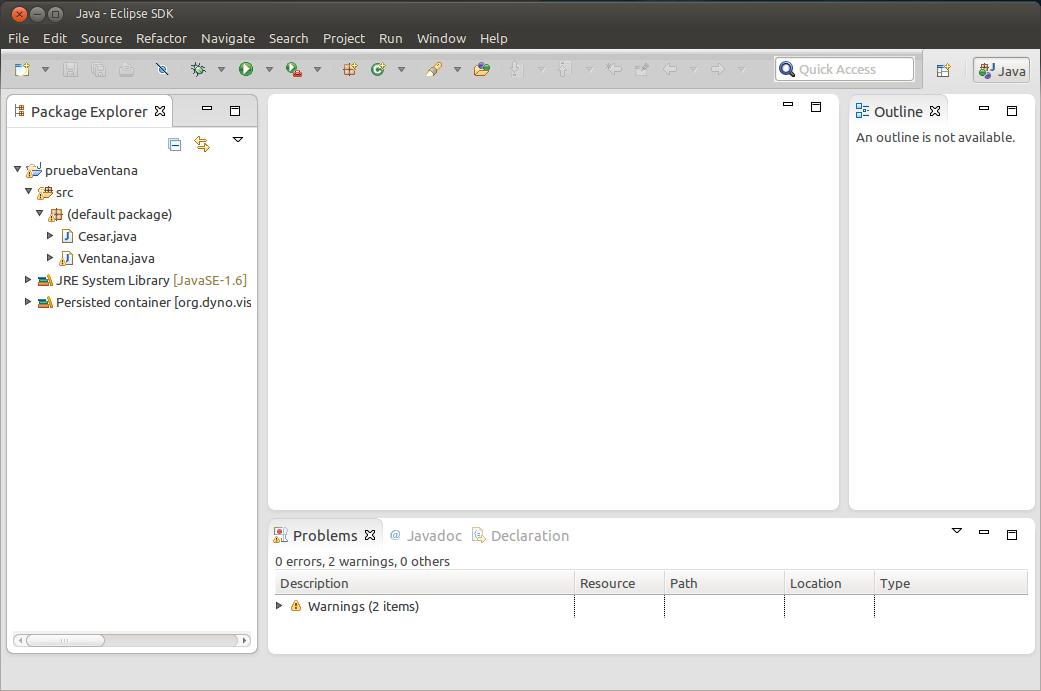
\includegraphics[scale=0.5]{./ConocimientosPrevios/imagenes/pantallaEclipse.png}
  \caption{Eclipse 4.2 Juno.}
  \label{fig:pantallaEclipse}
\end{figure} 

En el proyecto hemos usado la versión \textbf{Indigo}, que equivale a la versión 3.7 de Eclipse.

\subsection{Historia}

Eclipse comenzó como un proyecto de IBM Canadá. En noviembre de 2001 se creó un grupo de empresas para promover el desarrollo de Eclipse como software libre, los miembros iniciales eran Borland, IBM, Merant, QNX Software Systems, Rational Software, Red Hat, SuSE, TogetherSoft and WebGain. Finalmente en enero de 2004 se creó la Eclipse Foundation. 

\subsection{Versiones}

\begin{itemize}

	\item \textbf{Versión 3.0} (21 de junio de 2004)
	
	\item \textbf{Versión 3.1} (28 de junio de 2005)
	
	\item \textbf{Versión 3.2} (30 de junio de 2006): recibió el nombre de Callisto.
	
	\item \textbf{Versión 3.3} (29 de junio de 2007): recibió el nombre de Europa.
	
	\item \textbf{Versión 3.4} (25 de junio de 2008): recibió el nombre de Ganymede.
	
	\item \textbf{Versión 3.5} (24 de junio de 2009): recibió el nombre de Galileo.
	
	\item \textbf{Versión 3.6} (23 de junio de 2010): recibió el nombre de Helios.
	
	\item \textbf{Versión 3.7} (22 de junio de 2011): recibió el nombre de Indigo.
	
	\item \textbf{Versión 4.2} (27 de junio de 2012): recibió el nombre de Juno.
	
	\item \textbf{Versión 4.3} (26 de junio de 2013): esta será la próxima versión, que saldrá el próximo año y recibirá el nombre de Kepler.

\end{itemize}

\section{Criptografía.}\label{lbl:criptografia}

La criptografía es la ciencia que se encarga del estudio y creación de técnicas para la protección de una comunicación, para que solamente los usuarios autorizados puedan verla, leerla y entenderla. En la actualidad la criptografía es un término que se usa de forma similar a encriptación, que es el proceso para transformar una información mediante diferentes algoritmos, en un mensaje que no pueda entender un atacante que intercepte una comunicación. 

En el proyecto hemos usado una criptografía llamada \textbf{Criptografía de Clave Pública}, que como veremos a continuación en la historia brevemente y posteriormente en el capítulo~\ref{cap:criptografia}, en el que se explicará la criptografía usada a lo largo del proyecto con mas profundidad, consta de dos claves, ambas enlazadas matemáticamente y si conocemos una no podremos de ninguna forma conseguir la otra. La pública es la que tendría la persona que quiera desencriptar el mensaje, que a su vez da nombre a este algoritmo y otra privada que sólo conocerá la persona que quiere encriptar el mensaje.

La criptografía ha evolucionado mucho y actualmente no solo se usan para proteger mensajes, si no que también se usa para proteger la integridad de ellos. Este es uno de los usos más común de la criptografía de clave pública.

\subsection{Historia}

Podemos hacer dos grandes grupos dentro de la historia de la criptografía, la criptografía clásica y la criptografía durante la época de los ordenadores.

\subsection{Criptografía clásica.}

	Durante la época de la criptografía clásica sólo se quería proteger el mensaje que se enviaba de la mirada de curiosos y enemigos por lo que únicamente existían algoritmos de encriptación, la integridad del mensaje no importaba en esa época.  
	
	En dicha época todos los algoritmos de cifrados que existían eran por transposición o sustitución de caracteres. A continuación exponer unos ejemplos de los algoritmos utilizados más famosos. 
\begin{itemize}

	\item \textbf{Cifrado Cesar:} dicho cifrado es famoso porque los usaban las centurias romanas para comunicarse entre ellas de manera que si un mensaje era interceptado no pudiera ser leído. Consiste en sustituir cada carácter del mensaje por el que hay tres lugares a la derecha. Por ejemplo si tenemos el mensaje ``Hola" si lo ciframos con este sistema conseguimos ``Krod", en la figura \ref{fig:cifradoCesar} podemos ver como es el cifrado.
	
	Para desencriptar solo habría que intercambiar por la tercera letra anterior.

\begin{figure}[h]
  \centering
    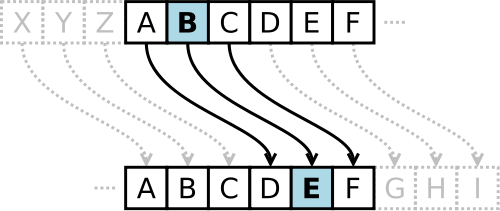
\includegraphics[scale=0.6]{./ConocimientosPrevios/imagenes/cifradoCesar.png}
  \caption{Ejemplo Cifrado Cesar}
  \label{fig:cifradoCesar}
\end{figure} 

	\item \textbf{Cifrado Homofónico:} Es una evolución del siguiente, pero en vez de sustituir siempre por el mismo carácter lo que se hace es tener la posibilidad de poder realizar varios cambios posibles, por lo que un mismo mensaje podría generar varios textos cifrados, complicando así su desencriptación. En la figura \ref{fig:cifradoHomofonico} podemos ver una tabla sencilla de sustitución para realizar el cifrado. Por ejemplo si ciframos la palabra ``PLATON" nos daría de resultado ``882110772963", pero podríamos sustituir la P no solo por 88 si no por cualquier valor de la tabla dando lugar a que pudiéramos crear varios mensajes cifrados.
	
\begin{figure}[h]
  \centering
    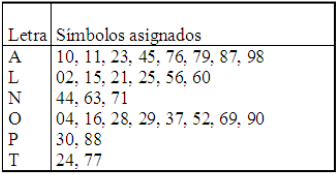
\includegraphics[scale=0.7]{./ConocimientosPrevios/imagenes/cifradoHomofonico.png}
  \caption{Tabla para cifrado homofónico}
  \label{fig:cifradoHomofonico}
\end{figure}

	\item \textbf{Cifrado por Transposición:} consiste en realizar una permutación de las posiciones que ocupan las letras escritas, un ejemplo podría ser escribir todo el texto con una cierta longitud preestablecida y luego leerlo por columnas en vez de por filas. En la figura \ref{fig:cifradoTransposicion} podemos ver un ejemplo del mecanismo de cifrado.  

\begin{figure}[h]
  \centering
    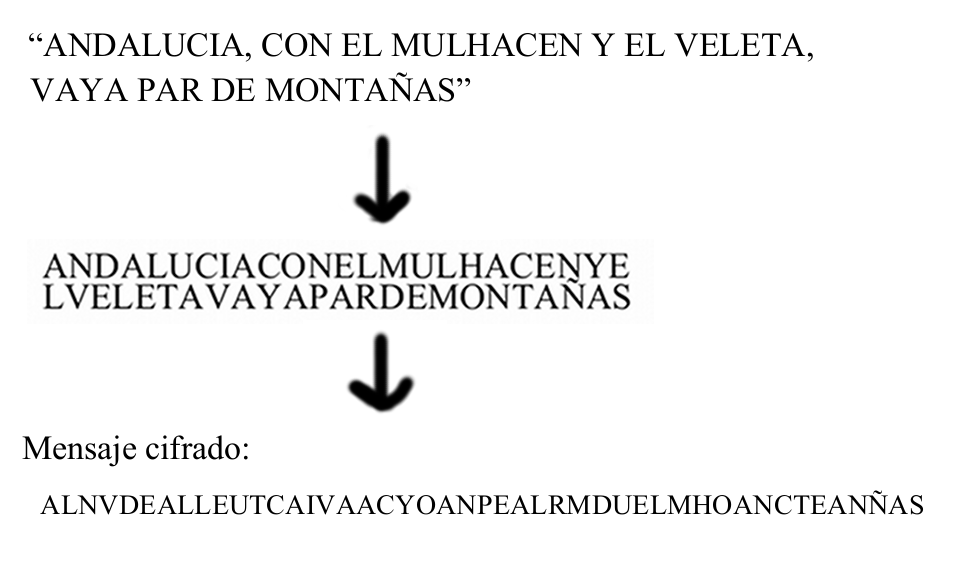
\includegraphics[scale=0.4]{./ConocimientosPrevios/imagenes/cifradoTransposicion.png}
  \caption{Ejemplo de cifrado por sustitución}
  \label{fig:cifradoTransposicion}
\end{figure}	

	\item \textbf{Cifrado Producto:} Es un cifrado que combina sustitución y transposición y se puede considerar como un encadenamiento de varios cifrados. Esto da lugar a cifrados complejos, seguros y difíciles de atacar, ya que tendríamos que averiguar no sólo el método de cifrado utilizado, sino que también tendríamos que saber el orden en el que se ha ejecutado las encriptaciones.

	\item \textbf{Cifrado Vernam:} es un tipo de cifrado que se denomina cifrado de flujo. El texto en claro se combina con una cadena, del mismo tamaño del texto en claro, de número aleatorios o pseudoaleatorio por medio de la función XOR. Lo inventó Gilbert Vernam que era un ingeniero de AT\&T en 1917. Es también conocido como RC4 en internet.  
	
\end{itemize}

\subsection{Criptografía durante la época de los ordenadores.}

La criptografía dio un gran salto en cuanto a calidad en el momento en el que se empezaron a usar ordenadores para encriptar y desencriptar textos, debido a que los ordenadores son máquinas que las tareas repetitivas las hacen muy bien y muy rápidos.

Se empezaron a idear nuevos algoritmos de cifrado mucho más complejos, los cuales se pueden dividir en dos grandes grupos, la criptografía de clave simétrica y la criptografía de clave pública. A continuación vamos a explicar brevemente los algoritmos más famosos de ambos.

\subsubsection*{Criptografía de Clave simétrica}

La principal característica de esta técnica de criptografía es que usan la misma clave para encriptar y desencriptar.

\begin{itemize}

	\item \textbf{Data Encryption Standard (DES):} Fue presentado por IBM en 1974, para generar un estandar de cifrado para transmisión de datos y cifrado de almacenamiento de datos y que fuera usado por gobiernos, empresas privadas o cualquier usuario. IBM comenzó el desarrollo basándose en un dispositivo de cifrado llamado Lucifer el cual tenia una clave de 128 bits. DES es un criptosistema de clave secreta que cifra en bloques de 64 bits del texto en claro y genera otros bloques de 64 bits del texto cifrado. La clave utilizada también es de 64 bits, pero el bit final de cada octeto de los 64 bits de la clave se usa como bit de paridad para control de errores. El cifrado se realiza en 16 iteraciones en las que se usan varias operaciones como son operaciones XOR, permutaciones y sustituciones. El esquema para cifrar se puede ver en la figura \ref{fig:cifradoDes}.
	
\begin{figure}
  \centering
    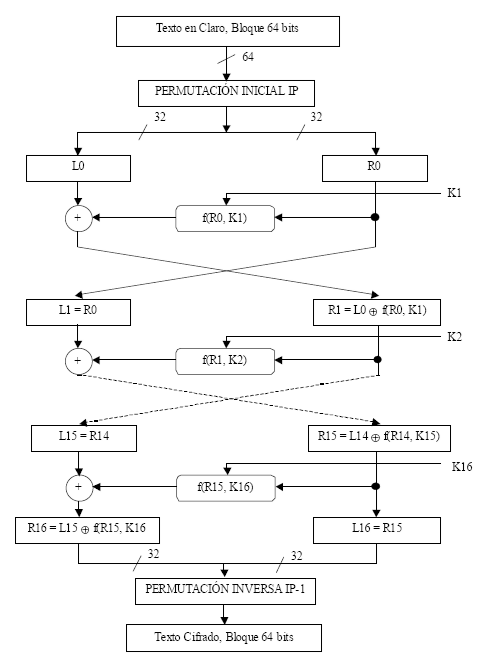
\includegraphics{./ConocimientosPrevios/imagenes/cifradoDes.png}
  \caption{Iteraciones en el cifrado DES}
  \label{fig:cifradoDes}
\end{figure}

\item \textbf{AES (Rijndael):} Fue presentado al concurso AES el 2 de enero de 1997 y anunciado ganador en 2001. Fue diseñado por dos criptólogos llamados Joan Daemen y Vincent Rijmen, ambos estudiantes de la Katholieke Universiteit Leuven de Bélgica. Al contrario que DES, AES es una red de sustituciones y permutaciones no una red de Feistel, se transformó en estándar efectivo el 26 de mayo de 2002 y en la actualidad es uno de los algoritmos de encriptación más famosos. Opera con bloques de 128 bits y tiene claves de 128, 192 y 256 bits.

\end{itemize}

El mayor problema que tiene este tipo de criptografía es que para que el destinatario pueda leer el mensaje necesita saber la clave y el intercambio de clave puede ser una dificultad muy grande si ambos usuarios no se pueden comunicar directamente, ya que usando cualquier otro método la clave podría ser interceptada y todo el proceso de encriptación sería inutil.

\subsubsection*{Criptografía de Clave Pública}

La criptografía de clave pública fue inventada por Diffie y Hellman y paralelamente por Merkle y ambos grupos aportaron a la criptografía el concepto de la utilización de pares de claves.

La característica principal es que cada usuario posee dos claves, una privada que sólo conoce el dueño de la clave y será usada para descifrar todo lo que otros usuarios cifren con su otra clave y otra la clave pública que es conocida por el resto de usuarios y será la que estos usarán para encriptar el mensaje que queremos que sea secreto. Así de esta forma si una persona quiere comunicarse con otra de forma secreta sólo tiene que conocer su clave pública, cifrar con ella y el destinatario podrá descifrar el mensaje con su clave privada. 

Otra característica es que las claves son imposibles de deducir una a partir de la otra, ambas claves son de una gran longitud y son generadas mediante exponenciación y/o productos de números primos grandes.

En los primeros años de existencia de la criptografía de clave pública se inventaron tres sistemas, Algoritmo de la mochila de Merkle-Hellman que fue roto, el esquema de McEliece que está considerado imposible de llevar a la práctica y un tercero que es el que explicaremos a continuación llamado RSA cuyo uso de ha impuesto actualmente.

\begin{itemize}

	\item \textbf{RSA:} Su nombre proviene de sus creadores que son Rivest, Shamir y Adleman y se basaron en la idea: \textit{``es muy fácil multiplicar dos números enteros primos grandes, pero extremadamente difícil hallar la factorización del producto"}, cuando inventaron el RSA en 1997. Es un algoritmo exponencial. Una característica de RSA es que tanto el mensaje, como el texto cifrado tienen que ser un código decimal, por lo que se tendría que usar el valor ASCII de la letra por ejemplo. Un ejemplo de uso sería el siguiente, lo primero que se debe de hacer antes de enviar el mensaje es acordar el algoritmo que se va a usar, lo siguiente el emisor cifra el mensaje usando la clave pública del receptor y se lo envía. Acto seguido el receptor descifra el mensaje que ha enviado el receptor usando su propia clave privada. La gran ventaja de este método es que en ningún momento la clave privada se tiene que enviar, por lo que solucionamos el gran problema que dijimos que tenían los algoritmos de cifrado simétrico, que antes de nada había que intercambiar la clave con la vulnerabilidad que eso implicaba. 

\end{itemize}

El algoritmo RSA será explicado con más profundidad en el capítulo~\ref{cap:criptografia}.

Los algoritmos de clave pública tienen un gran problema, es que son muy lentos realizando el proceso de cifrado y descifrado, por lo que en la situaciones reales se usan para realizar el intercambio de claves de algoritmos de clave simétrica que son mucho más rápidos y también igual de seguros, de esta forma solucionamos su principal problema.

\section{Android.}

Android es un sistema operativo basado en Linux especialmente diseñado para smartphone, tablet, smart TV y una infinidad de dispositivos, desarrollado por Google con Open Handset Alliance. Android empezó siendo desarrollado por la compañía llamada Android que inicialemente fue financiada y después comprada por Google en 2005. En 2007 cuando se presentó por primera vez Android también se anunció la fundación de Open Handset Alliance que es un conjunto de 86 empresas, entre las que hay compañías de hardware, software y telecomunicaciones, interesadas en el mundo de los dispositivos móviles. Android es código abierto y está distribuido bajo licencia Apache\footnote{ Para saber más sobre la licencia visite: \url{http://en.wikipedia.org/wiki/Apache\_License}}. La tarea del mantenimiento y desarrollo de Android es de Android Open Source Project (AOSP).

Android tiene una gran comunidad de desarrolladores que pueden extender las funcionalidad de los teléfonos o de cualquier dispositivos que pueda ejecutar la máquina virtual de Android, se puede desarrollar tanto en Java usando el SDK o en C++ usando el NDK, posee una tienda online llamada Google Play (anteriormente Android Market), donde se pueden comprar aplicaciones, películas, libros o música y en la que cualquier desarrollador por una pequeña cantidad de dinero (alrededor de 25\euro, por una cuenta vitalicia de desarrollador) puede subir todas las aplicaciones gratuitas o de pago que desee. En Junio de 2012 había alrededor de 600.000 aplicaciones en Google Play.

En el primer cuatrimestre de 2012, Android tenía el 59\% del mercado de smartphones en el mundo, de ahí la importancia de esta plataforma para los desarrolladores, ya que proporciona un mercado muy amplio y una forma muy fácil y barata de conseguir un gran número de usuarios.

Los detalles técnicos de Android se explicarán con más profundidad en el capítulo~\ref{cap:android}.

\subsection{Historia.}

Como hemos dicho anteriormente Android fue diseñado y creado originalmente por una compañía llamada Android que fue fundada en Palo Alto, California en 2003 por Andy Rubin, Rich Miner, Nick Sears y Chris White. Originalmente solo estaba diseñado para funcionar con smartphones, ya que ellos pensaban que un smartphone era algo más que un dispositivo que sirviera para usar el GPS y tener preferencias. 

Google compró Android el 17 de agosto de 2005, con la intención de entrar en el mercado de los teléfonos móviles. Después de varios años de rumores el 5 de noviembre de 2007, Google presentó la Open Handset Alliance, un grupo de empresas que incluian a Broadcom Corporation, Google, HTC, Intel, LG, Marvell Technology Group, Motorola, Nvidia, Qualcomm, Samsung Electronics, Sprint Nextel, T-Mobile and Texas Instruments entre otras muchas empresas que estaban interesadas en generar estándares para dispositivos móviles. Ese mismo día también se lanzó el primer producto Android basado en el kernell de Linux 2.6.

Android ha sido muy criticado por la gran fragmentación que tiene debido al gran número de versiones que posee, que son compatibles hacia versiones abajo pero no hacia versiones posteriores, esto quiere decir que la versión 4.0 es compatible con todo el software que funcionase con las versiones 2.0, 2.3 o cualquiera inferior, pero no será compatibles con el software diseñado para la versión 4.1. Este problema hace necesario que los fabricantes actualicen el software de sus teléfono, lo que es un gran problema debido a que muchos no lo hacen, hubo un pequeño intento de solucionar esta problemática haciendo que los fabricantes estuvieran obligados a actualizar sus terminales al menos en los 18 meses posteriores a la salida al mercado, pero no hubo ningún acuerdo.   

\subsection{Versiones.}

Como curiosidad todas las versiones de Android se denominan con un nombre en clave que es un postre.
\begin{itemize}

	\item \textbf{1.0 (Apple Pie):} primera versión lanzada el 23 de septiembre del 2008.
	
	\item \textbf{1.1 (Banana Bread):} lanzada el 9 de febrero del 2009.
	
	\item \textbf{1.5 (Cupcake):} fue presentada el 30 de abril del 2009, esta fue la primera versión con la que Android empezó a despuntar y entrar en el mundo de los teléfonos móviles, anteriormente apenas si era conocido. Tenía características nuevas muy interesantes como poder grabar y reproducir vídeo, podía subir videos a Youtube e imágenes a Picasa directamente desde el teléfono, un nuevo teclado predictivo, nuevos widget y carpetas para colocar en la pantalla de inicio y transiciones animadas.

	\item \textbf{1.6 (Donut):} fue presentada el 15 de septiembre de 2009. Se le añadieron las siguientes características nuevas como una interfaz integrada para la cámara, la grabadora de vídeo y la galería, se actualizó la búsqueda por voz añadiendo soporte a más aplicaciones nativas y la posibilidad de llamar a contactos, se añadió un buscador general en la pantalla de inicio donde se podía buscar contactos, historiales y páginas web, se añadió un nuevo framework de gestos y las herramientas de desarrollo llamado GestureBuilder.

	\item \textbf{2.0 / 2.1 (Eclair):} la versión 2.0 fue presentada el 26 de octubre de 2009 y la 2.1 fue liberada el 3 de diciembre del 2009. Se añadieron un gran número de mejoras, se optimizó la velocidad de hardware, se soportaron más tamaño de pantallas y resoluciones, se rediseñó la interfaz de usuario, el navegador también fue renovado y se le añadió soporte para HTML5, nueva lista de contactos, se añadió soporte para el flash de la cámara, zoom digital, soporte para bluetooth 2.1, se mejoraron la captura de eventos multi-touch con MotionEvent y fondos de pantalla animados.
	
	\item \textbf{2.2 (Froyo):} fue lanzada el 20 de mayo de 2010. Se optimizó el sistema Android, la memoria y el rendimiento, se mejoró la velocidad de las aplicaciones gracias a la implementación de JIT, se implementó el motor JavaScript V8 de Google Chrome en el navegador del móvil, nueva funcionalidad de WiFi hotspot y tethering por USB, se actualizó el Android market para que tuviera actualizaciones automáticas, marcación por voz y compartir contactos por Bluetooth, soporte para contraseñas numéricas y alfanuméricas, soporte para Adobe Flash 10 y soporte para pantallas de HDPI, como pueden ser pantallas de 4" y resolución de 720p. 

	\item \textbf{2.3 (Gingerbread):} fue presentado el 6 de diciembre del 2010. Cambiaron el diseño de la interfaz de usuario, añadieron soporte para pantallas extra grandes y resoluciones WXGA, soporte nativo para VoIP SIP, reproducción nativa de vídeos WebM/VP8 un formato de vídeo patrocinado por Google que es la alternativa al H264 en la reproducción de vídeo en HTML5 y decodificación de audios en AAC, se añadió soporte a NFC (Near Field Communication), nuevo teclado multitáctil, soporte mejorado para programar en código nativo, soporte nativo de más sensores como pueden ser acelerómetros o barómetros, soporte para múltiples cámaras y cambio del sistema de archivos YAFFS a ext4. La versión 2.3.3 sigue siendo la versión de Android más usada actualmente. 

	\item \textbf{3.0 / 3.1 / 3.2 (Honeycomb):} Esta versión fue diseñada exclusivamente para tablet, por lo que no hubo smartphones que actualizaran a esta versión. Las características principales fueron un escritorio en 3D con widget rediseñado, sistema multitarea mejorado, mejoras en el navegador de internet, videochat mediante Google Talk, mejoras en el soporte de redes WiFi, añadidos soporte para gran cantidad de periféricos y conexión USB.
	
	\item \textbf{4.0 (Ice Cream Sandwich):} Fue una de las actualizaciones más importantes que ha recibido Android y fue lanzada el 19 de octubre de 2011, en ella se unificaron todas las versiones y se tenía una sola versión para smartphne, televisores, tablets, netbooks, etc. Se añadió una nueva versión de interfaz mucho más limpia y usable llamada Holo, una nueva fuente llamada Roboto, se da la opción de utilizar botones virtuales en la interfaz de usuario en vez de botones físicos, soporte para aceleración gráfica por hardware, por lo que la interfaz es manejada y dibujada por la GPU, aumentando notablemente el rendimiento, multitarea mejorada, se ha añadido un nuevo corrector ortográfico, en la lista de notificaciones se pueden eliminar las que no sean interesantes, capturas de pantalla pulsando el botón de encendido y el de bajar volumen, mejorada la aplicación encargada de hacer fotografías, añadida una nueva opción para crear fotos panorámicas, Android Beam, una nueva característica que nos permite compartir contenidos entre teléfonos mediante NFC, reconocimiento de voz del usuario, reconocimiento facial, para bloqueo y desbloqueo del teléfono, añadidas nuevas carpetas que se crean sólo con arrastrar y soltar, un único y nuevo framework para crear aplicaciones y soporte para contenedor MKV.

	\item \textbf{4.1 (Jelly Bean):} Esta es la última versión de Android que hay en el mercado, fue lanzada el 27 de junio de 2012 durantes la última Google I/O. Se mejoró la fluidez y la estabilidad gracias al proyecto ``Project Butter", ajuste automático de widget cuando se añaden al escritorio, se añadió soporte para lenguas no occidentales, mejora de Android Beam para poder enviar video por NFC, dictado de voz mejorada y sin tener que tener conexión a internet para usarlo, nuevas notificaciones en las que se puede añadir botones para controlar o tener acceso a opciones más comunes, como puede ser responder a un email, pulsar pause o pasar de canción, nueva función Google Now que intenta ser el competidor de SIRI del iPhone en Android, cifrado de aplicaciones y nuevas actualizaciones incrementales, en las que no es necesario volver a bajar toda la aplicación para actualizarla, sólo se baja las partes nuevas, Google Chrome se convierte en el navegador por defecto de Android y se pone fin al soporte de Adoble Flash Player, se añade una nueva función llamada Sound Search que permite identificar la canción que está sonando, se ha añadido una nueva función llamada Gestual Mode para personas discapacitadas visualmente.
\end{itemize}

En el proyecto se ha usado la versión \textbf{Android 4.0} para el desarrollo.

En la figura \ref{fig:Android41} se puede ver como es visualemte Android en la actualidad, con la versión 4.1.

\begin{figure}
  \centering
    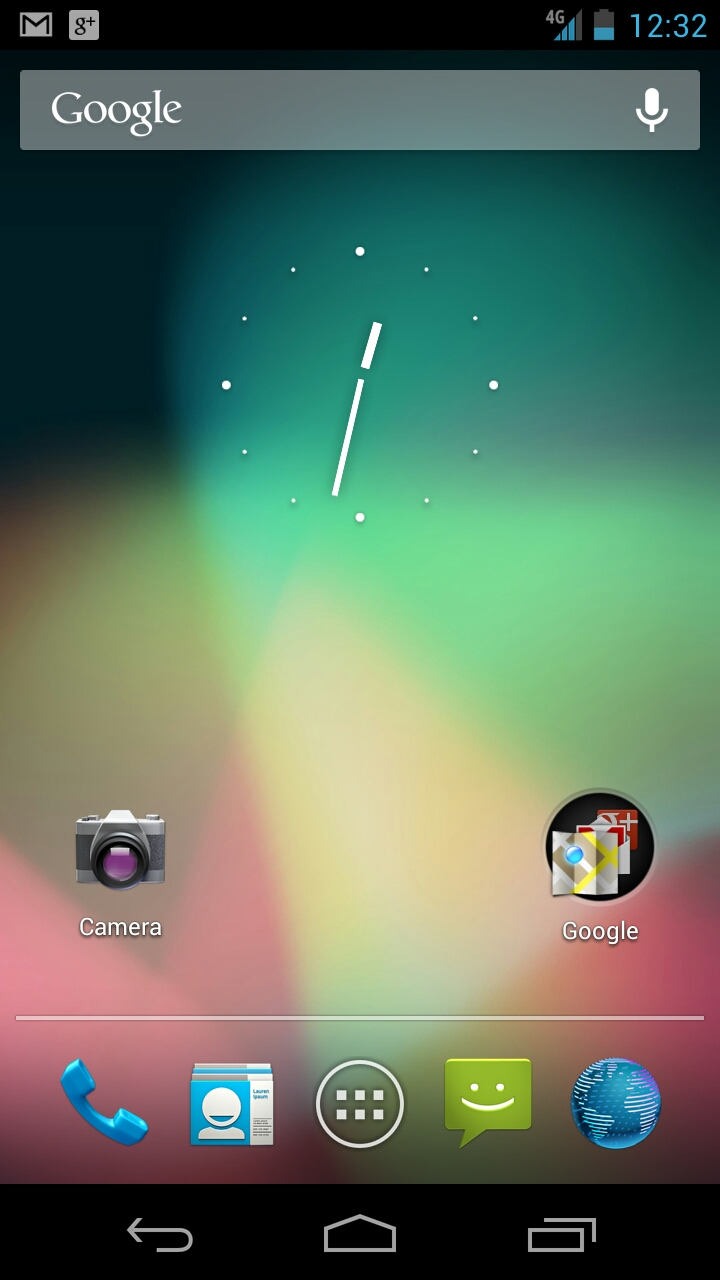
\includegraphics[scale=0.2]{./ConocimientosPrevios/imagenes/android41.jpeg}
  \caption{Versión de Android 4.1}
  \label{fig:Android41}
\end{figure}


\section{Google App Engine.}

Google App Engine es una plataforma de cloud computing para desarrollar y almacenar aplicaciones web que ofrece Google. Las aplicaciones web pueden ser escalables y si necesitan más recursos automáticamente le son asignados para poder seguir ofreciendo servicio. Google App Engine es gratis para un cierto número de peticiones y almacenamiento y la primera versión fue lanzada en abril de 2008.

Actualmente se puede desarrollar en tres lenguajes, que son Java, Python y Go, este último un lenguaje creado por Google. En el proyecto hemos usado Java para desarrollar en la plataforma. 

Google App Engine para Java soporta muchos estándares y framework, y el Core está hecho con la tecnología Servlet 2.5 usando el servidor de software libre llamado Jetty Web Server, acompañado con otras tecnologías como JSP. El almacén de datos puede ser muy poco intuitivo desde el punto de vista de los desarrolladores, pero se puede acceder fácilmente con JPA (Java Persistence API) y los métodos JDO (Java Data Objects) para escritura y lectura de datos. También se pueden usar tecnologías como Spring Framework.

Google garantiza que aplicación estará disponible el 99.95\% del tiempo, para ello ofrece una alta replicación.

La base de datos a la que nos dan acceso no es una base de datos estándar, como pueden ser MySQL, Oracle o SQLServer, pero tiene una sintaxis muy parecida a SQL, llamada GQL. Una de las principales diferencias es que no admite sentencias join, debido a la ineficiencia de la misma. La versión de Java soporta consultas asíncronas no bloqueantes, ofreciendo así una forma de procesamiento paralelo de datos.

Para más información se puede visitar la web diseñada para desarrolladores que proporciona Google, \url{https://developers.google.com/appengine/}. 

En el capítulo \ref{cap:GAE} veremos más ampliamente todo lo relacionado con Google App Engine que hemos usado en el proyecto.

\section{SQLite.}

SQLite es un sistema gestión de base de datos relacionales compatibles con ACID, ACID es el acrónimo de Atomicity, Consistency, Isolation and Durability, que son las características que debe tener una base de datos para que se consideren base de datos relacional. Su característica principal es que ocupa muy poco espacio, alrededor de 275 Kb y fue escrita en el lenguaje C por Richard Hipp. Está distribuida bajo licencia de dominio público.

A diferencia de los sistemas de gestión de base de datos clientes-servidor, el motor de SQLite pasa a ser parte del programa que quiere usarlo, ya que se integra con él. Esto hace que tenga mayor rendimiento debido a que la comunicación es por medio de funciones, que es mucho más eficiente que mediante comunicación de procesos. La totalidad de la base de datos, tablas, índices y datos, se guardan en un solo fichero estándar en la máquina host. La versión 3 de SQLite permite base de datos de hasta 2 Terabytes y permite campos del tipo BLOB.

SQLite está muy extendido y se puede programar en infinidad de lenguajes de programación como pueden ser C, C++, Perl, Python, PHP, Java, etc.

Es utilizado en infinidad de programas y sistemas, que van desde editores de imagen como puede ser Adobe Photoshop Elements, reproductores de sonido como Clementine o navegadores como Firefox, Chrome u Opera.

Esta es una de las tres formas que proporciona Android para guardar datos, al estar embebida en cada aplicación para mejorar el rendimiento, cada aplicación debe de tener una. 

\section{XML.}

XML son las siglas en inglés de e\textbf{X}tensible \textbf{M}arkup \textbf{L}anguage que es un lenguaje de marcas desarrollado por el World Wide Web Consortium (W3C), deriva del lenguaje SGML y permite definir la gramática de lenguajes específicos para estructurar documentos grandes.

Es una de las formas de intercambio estructurado de información más extendidas en internet, ya que se puede usar en base de datos, hojas de cálculo o en casi cualquier información que se quiera usar.

XML es un lenguaje que puede ser analizado sintácticamente para averiguar si está bien construido o no, por lo que cualquier parser (analizador sintáctico) puede confirmar si tiene la estructura bien definida según el estándar. Todos los documentos tiene que tener las siguientes partes: prólogo, cuerpo, elementos y atributos.

Un ejemplo podemos verlo en el siguiente un trozo de código XML, para almacenar un libro en una librería.

\begin{lstlisting}[language=XML]   
<?xml version="1.0"?>
<libro>
<titulo> A Game of Thrones </titulo>
<disponible tiempo="24" unidad="horas"/>
<autor> George R. R. Martin </autor>
<formato> Rústica </formato>
<publicacion> 1996 </publicacion>
<precio cantidad="9.99" moneda="euro"/>
<descuento cantidad="5"/>
<enlacelibro href="/exec/ISBN/0-553-10354-7"/>
</libro>
\end{lstlisting}

En el proyecto hemos usado XML, en los archivos de configuración o para el diseño de las interfaces en Android. En una de la aplicaciones web realizadas para los archivos de configuración también hemos usado XML, en la otra hemos usado un lenguaje parecido llamado YALM, que es equivalente a XML.

\section{UML.}

UML es un lenguaje de modelado de propósito general más usado en la actualidad para el diseño de software. UML son las siglas de Unified Modeling Language. UML tiene la ventaja de que se puede observar visualmente el diseño del software. Se puede desde especificar, construir o documentar un sistema o un software.

\begin{figure}
  \centering
    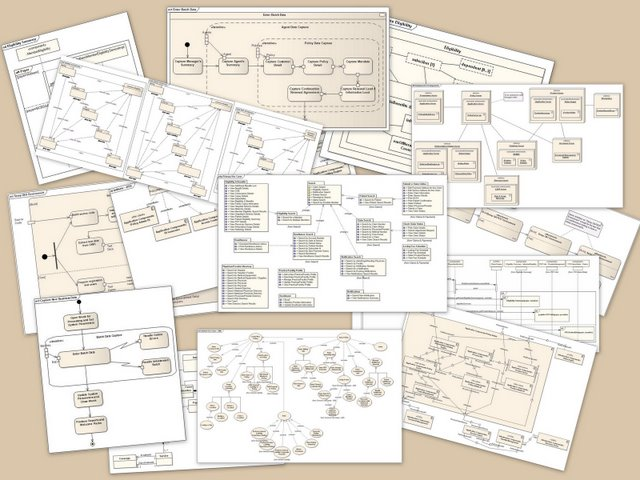
\includegraphics[scale=0.4]{./ConocimientosPrevios/imagenes/UMLDiagrams.jpg}
  \caption{Ejemplos de diseños realizados con UML.}
  \label{fig:UMLDiagrams}
\end{figure}

En la figura~\ref{fig:UMLDiagrams} podemos ver los diferentes diagramas que podemos realizar mediantes UML.

Hemos usado UML para diseñar las clases usadas a lo largo de todo el proyecto, además de para mostrar en la memoria del proyecto la relación de las clases, los casos de uso, etc.

\section{GIT.}

Git es un software de control de versiones, a la vez que mantenedor de la coherencia y cohesión del código fuente orientado a la velocidad. Fue desarrollado para el manejo del código fuente de Linux y al principio fue diseñado por Linus Torvalds. GIT es un repositorio con un completo historial y una capacidad de identificación de cada cambio realizado sin depender del acceso a la red o a un servidor central. Está liberado con licencia GNU versión 2.

En el proyecto hemos estado usando GIT como control de versiones, ya que si en algún cambio ocurría algún problema poder volver atrás y para tener una copia de seguridad del proyecto, alojado en todo momento en un servidor externo por si ocurría algún problema en el ordenador donde desarrollamos el proyecto.

A lo largo del proyecto hemos usado dos servicios gratuitos  que proporcionan servidores GIT, como pueden ser \url{https://github.com/} y \url{https://bitbucket.org/}. El primero es muy conocido actualmente y hay una gran comunidad de software libre en dicha plataforma, tiene un pequeño problema para nuestro proyecto y es que el código tiene que ser libre y en la versión gratuita no se pueden tener repositorios privados, cosa que el segundo servicio si te lo ofrece. Para todo el código fuente usando, tanto en la aplicación de Android como en las dos aplicaciones hemos usado bitbucket y para la memoria de proyecto hemos usado github. La dirección del repositorio de la memoria es la siguiente: \url{https://github.com/t321/memoriaPFC}, el repositorio de las aplicaciones web \url{https://bitbucket.org/t321/pfcaeg} y el de la aplicación de Android \url{https://bitbucket.org/t321/pfcandroid}.

La configuración básica para el uso de GIT con Eclipse se puede ver en el apendice~\ref{cap:apendiceA}.  














